\documentclass[xcolor=table]{beamer}
\usetheme{Antibes}

\usepackage[utf8x]{inputenc}
%\usepackage{helvet}
\usepackage{color}
\usepackage{graphicx}
\usepackage{hyperref}
\usepackage[outputdir=build]{minted}
\usepackage{pgfplots}
\usemintedstyle{monokai}
\usepackage{tikz}
\usetikzlibrary{positioning,shapes, arrows,decorations.pathmorphing,mindmap,trees}

\definecolor{softgreen}{RGB}{34, 139, 34} % ForestGreen

% Changer la couleur principale en vert
\usecolortheme[named=softgreen]{structure}

% Changer le fond de la barre laterale en vert
\setbeamercolor{sidebar right}{bg=softgreen}
\setbeamercolor{sidebar left}{bg=softgreen}

% Changer la couleur des titres
\setbeamercolor{title}{fg=white,bg=softgreen}
\setbeamercolor{frametitle}{fg=white,bg=softgreen}



\setbeamertemplate{footline} {
\hspace{8cm}
Ph0wn Labs 2025 - A. Apvrille
\insertframenumber/\inserttotalframenumber
%\vspace{0.2cm}
}

\setbeamertemplate{blocks}[rounded][shadow=true]
\setbeamertemplate{itemize item}[square]
\setbeamertemplate{enumerate items}[circle]

\setbeamertemplate{navigation symbols}{}



\hypersetup{
%      pdfpagemode = FullScreen,% afficher le pdf en plein écran
      pdfauthor   = {Axelle Apvrille},
      pdftitle    = {Ph0wn Labs 01},
      pdfcreator  = {PDFLaTeX},%
      pdfproducer = {PDFLaTeX},%
      colorlinks=true
}


\title{\textbf{Radare2}}
\author{Axelle Apvrille, Fortinet}
\date{Ph0wn Labs, February 13, 2025}

\begin{document}


% Title slide ---------------
\frame[plain]{
\titlepage
}


\section{Introduction}

\frame{
  \frametitle{Who am I?}
  \centering
  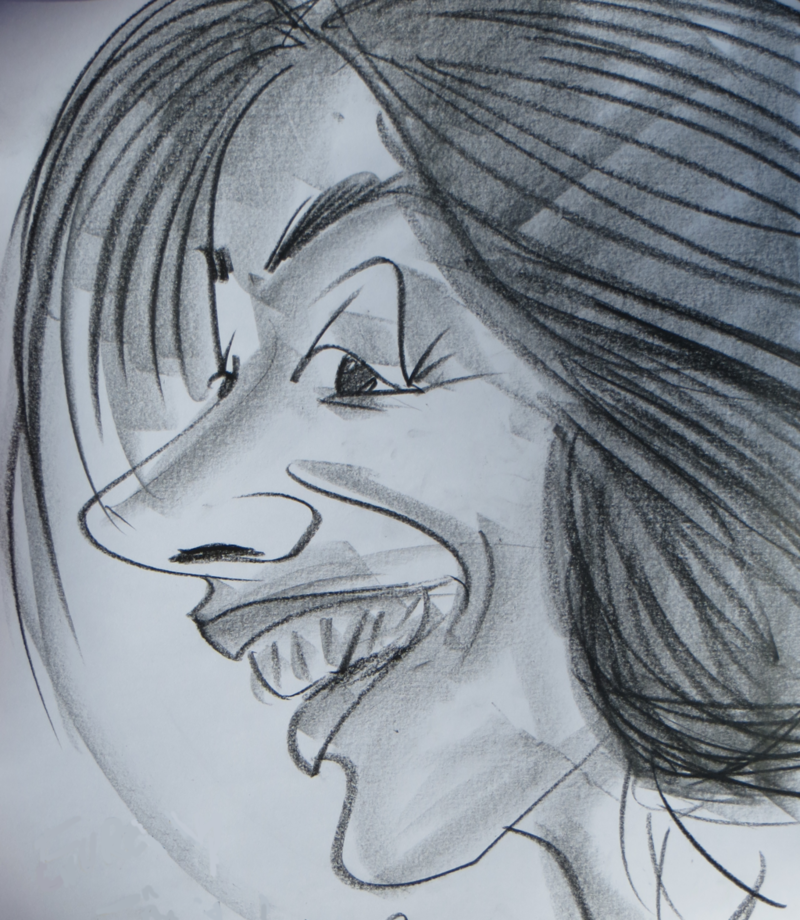
\includegraphics[height=4cm]{./images/caricature-ax.png}\\
  Officially known as \textbf{Axelle} or \textbf{Cryptax}.\\
  Malware analysis and Research on Android and IoT \textbf{malware} at \textbf{Fortinet}.\\
  I morph in a \textit{crocodile named Pico le Croco}\\
}

\frame{
  \frametitle{What is Ph0wn?}

  \centering
  
\includegraphics[width=5cm]{./images/logo-ph0wn.png}\\
  \url{https://ph0wn.org}\\
  Hacking challenges for embedded systems, IoT, smartphones...\\
  Once per year - Next in \textbf{March 2026} (in 1 year)\\
  On site: Sophia Antipolis\\
  + Free workshops\\

}

\frame{
  \frametitle{Want to talk? contribute? sponsor?}
  \centering
  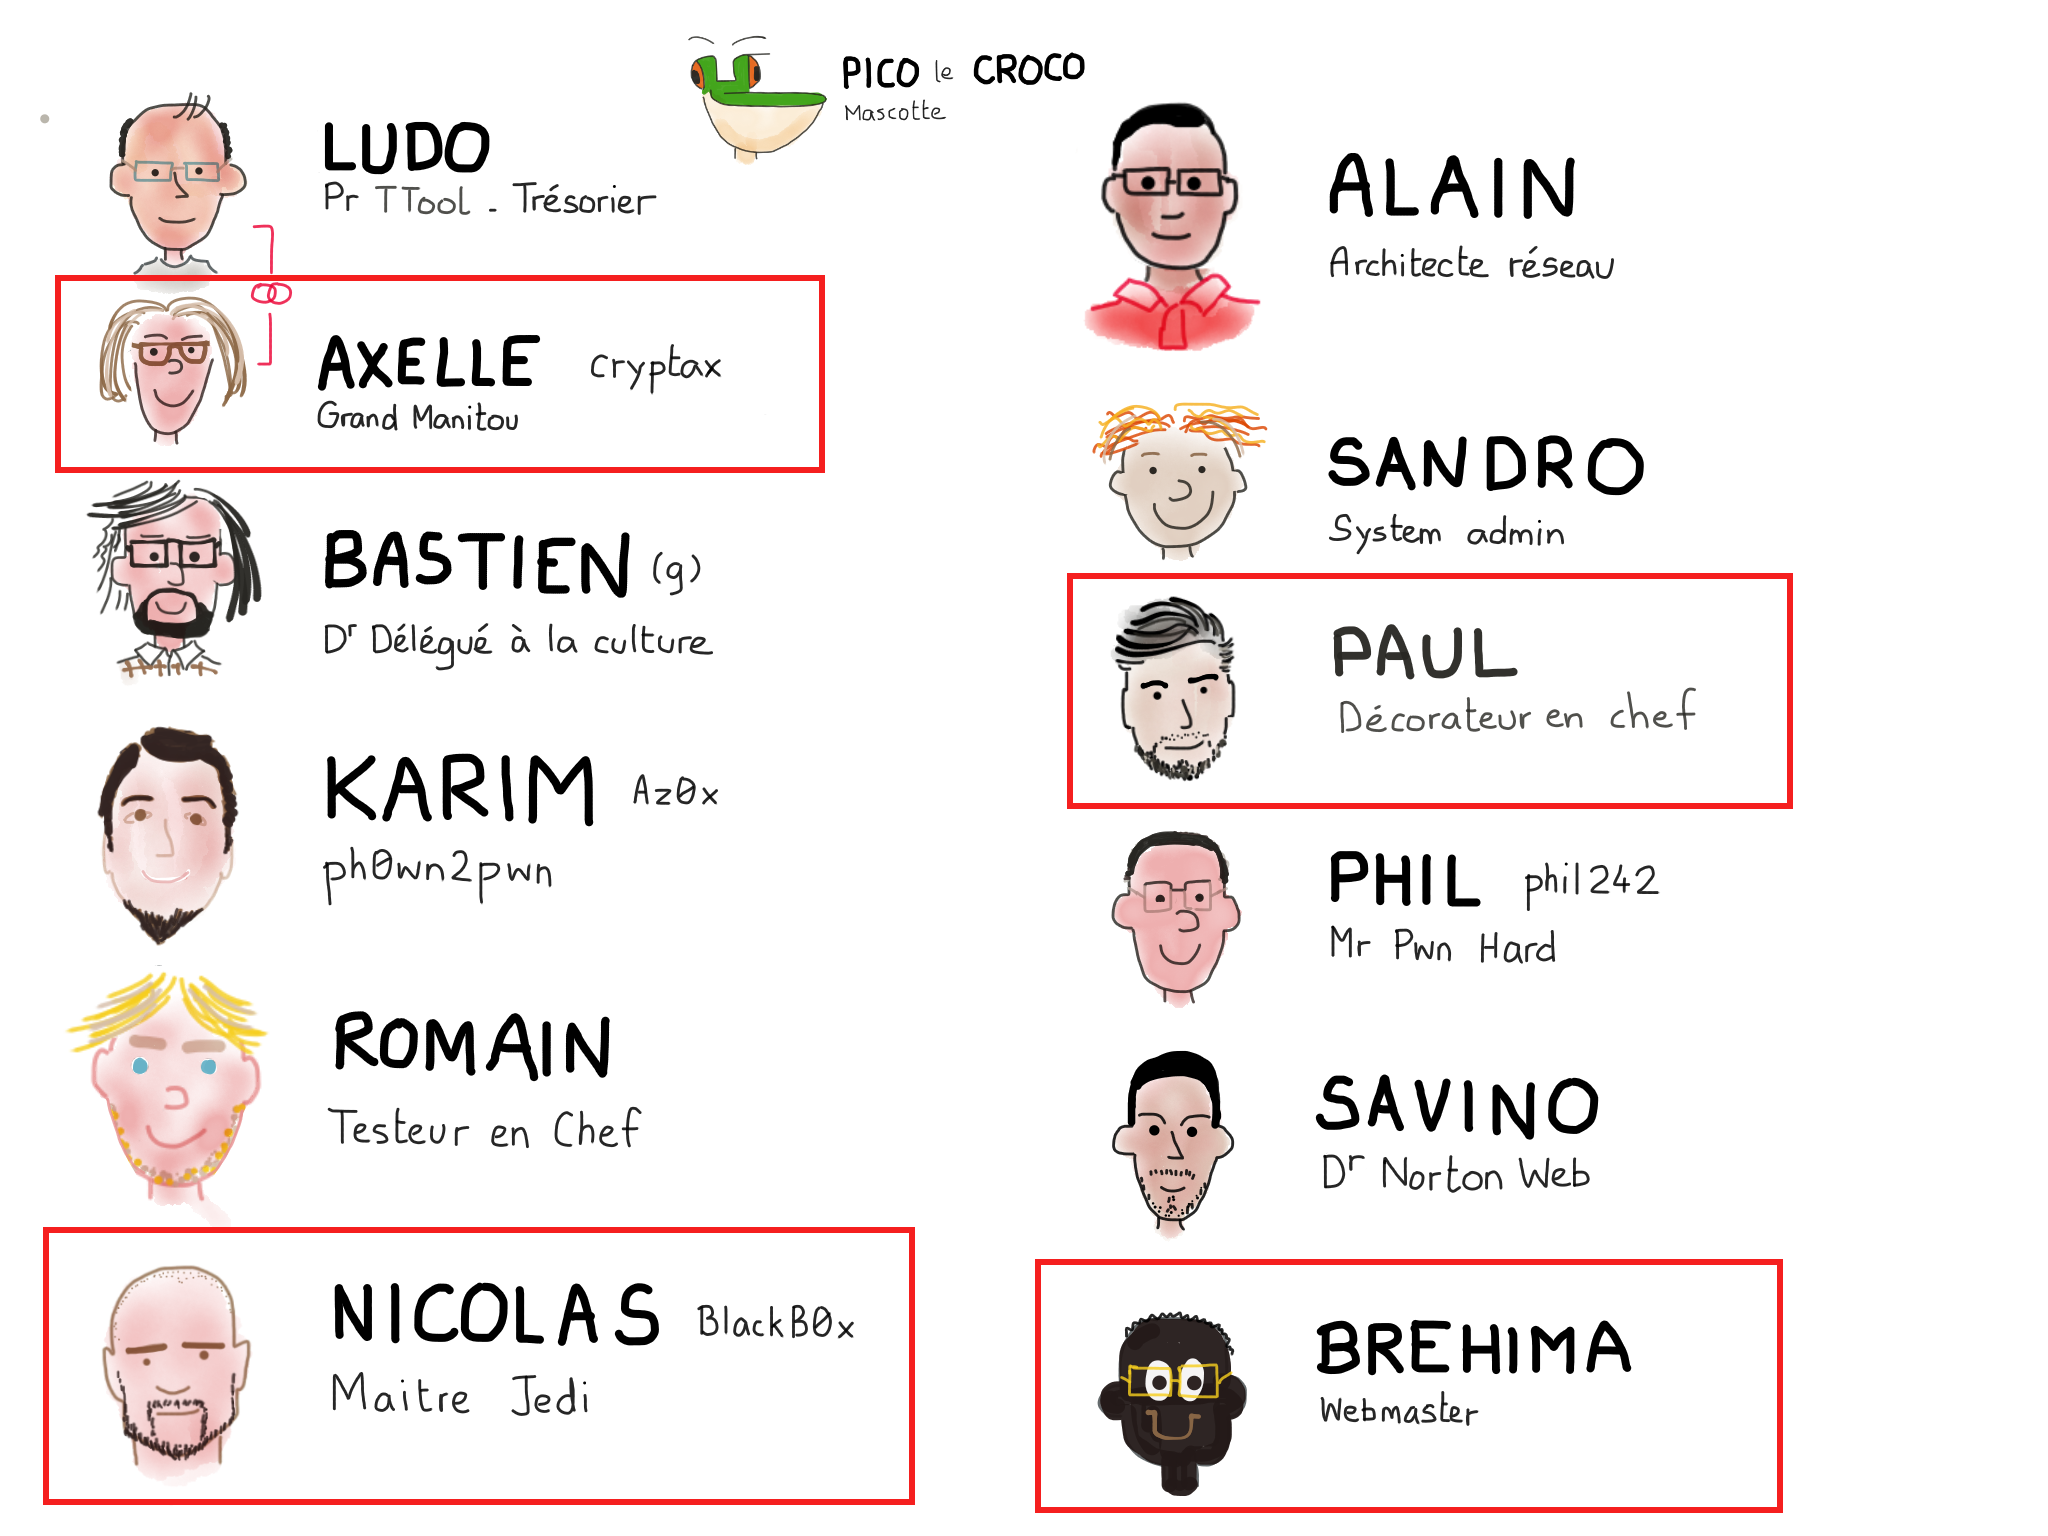
\includegraphics[height=7cm]{./images/organizers.png}
}



\frame{
  \frametitle{What are Ph0wn Labs?}

  \begin{columns}
    \column{6cm}
    \centering
    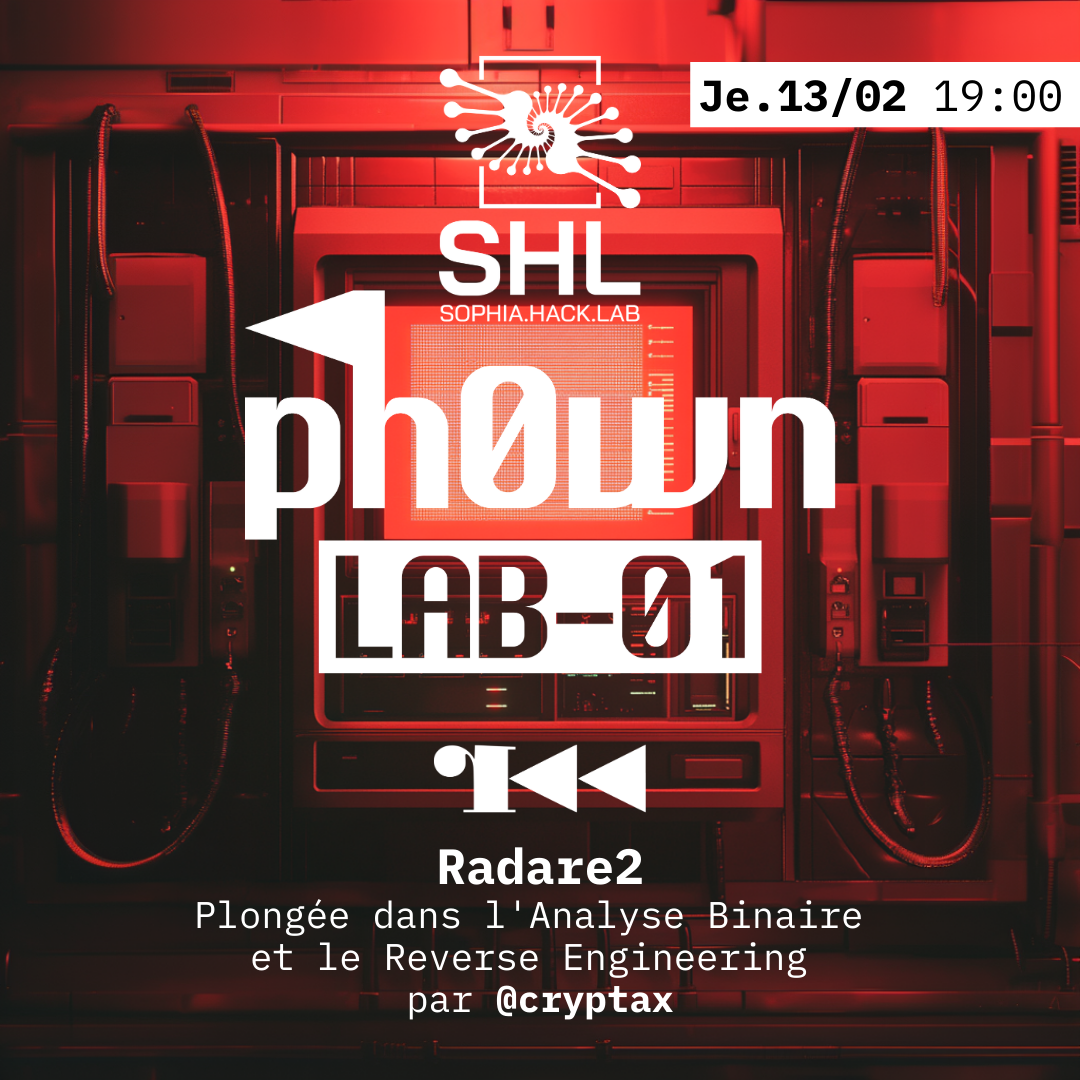
\includegraphics[width=5cm]{../../images/ph0wn.Labs_LAB-01.png}\\
    \column{6cm}
    \begin{itemize}
      \item SHL/Ph0wn initiative to train on Jeopardy CTFs
      \item   Re-play Ph0wn challenges
      \item Play other CTFs: \url{https://ctftime.org}
      \item Discuss IoT, retro-gaming, reverse etc
      \item Expect every 2 months?
    \end{itemize}
    \end{columns}
}

\section{Lab 01}

\frame{
  \frametitle{Agenda for Ph0wn Lab 01}
  \centering
  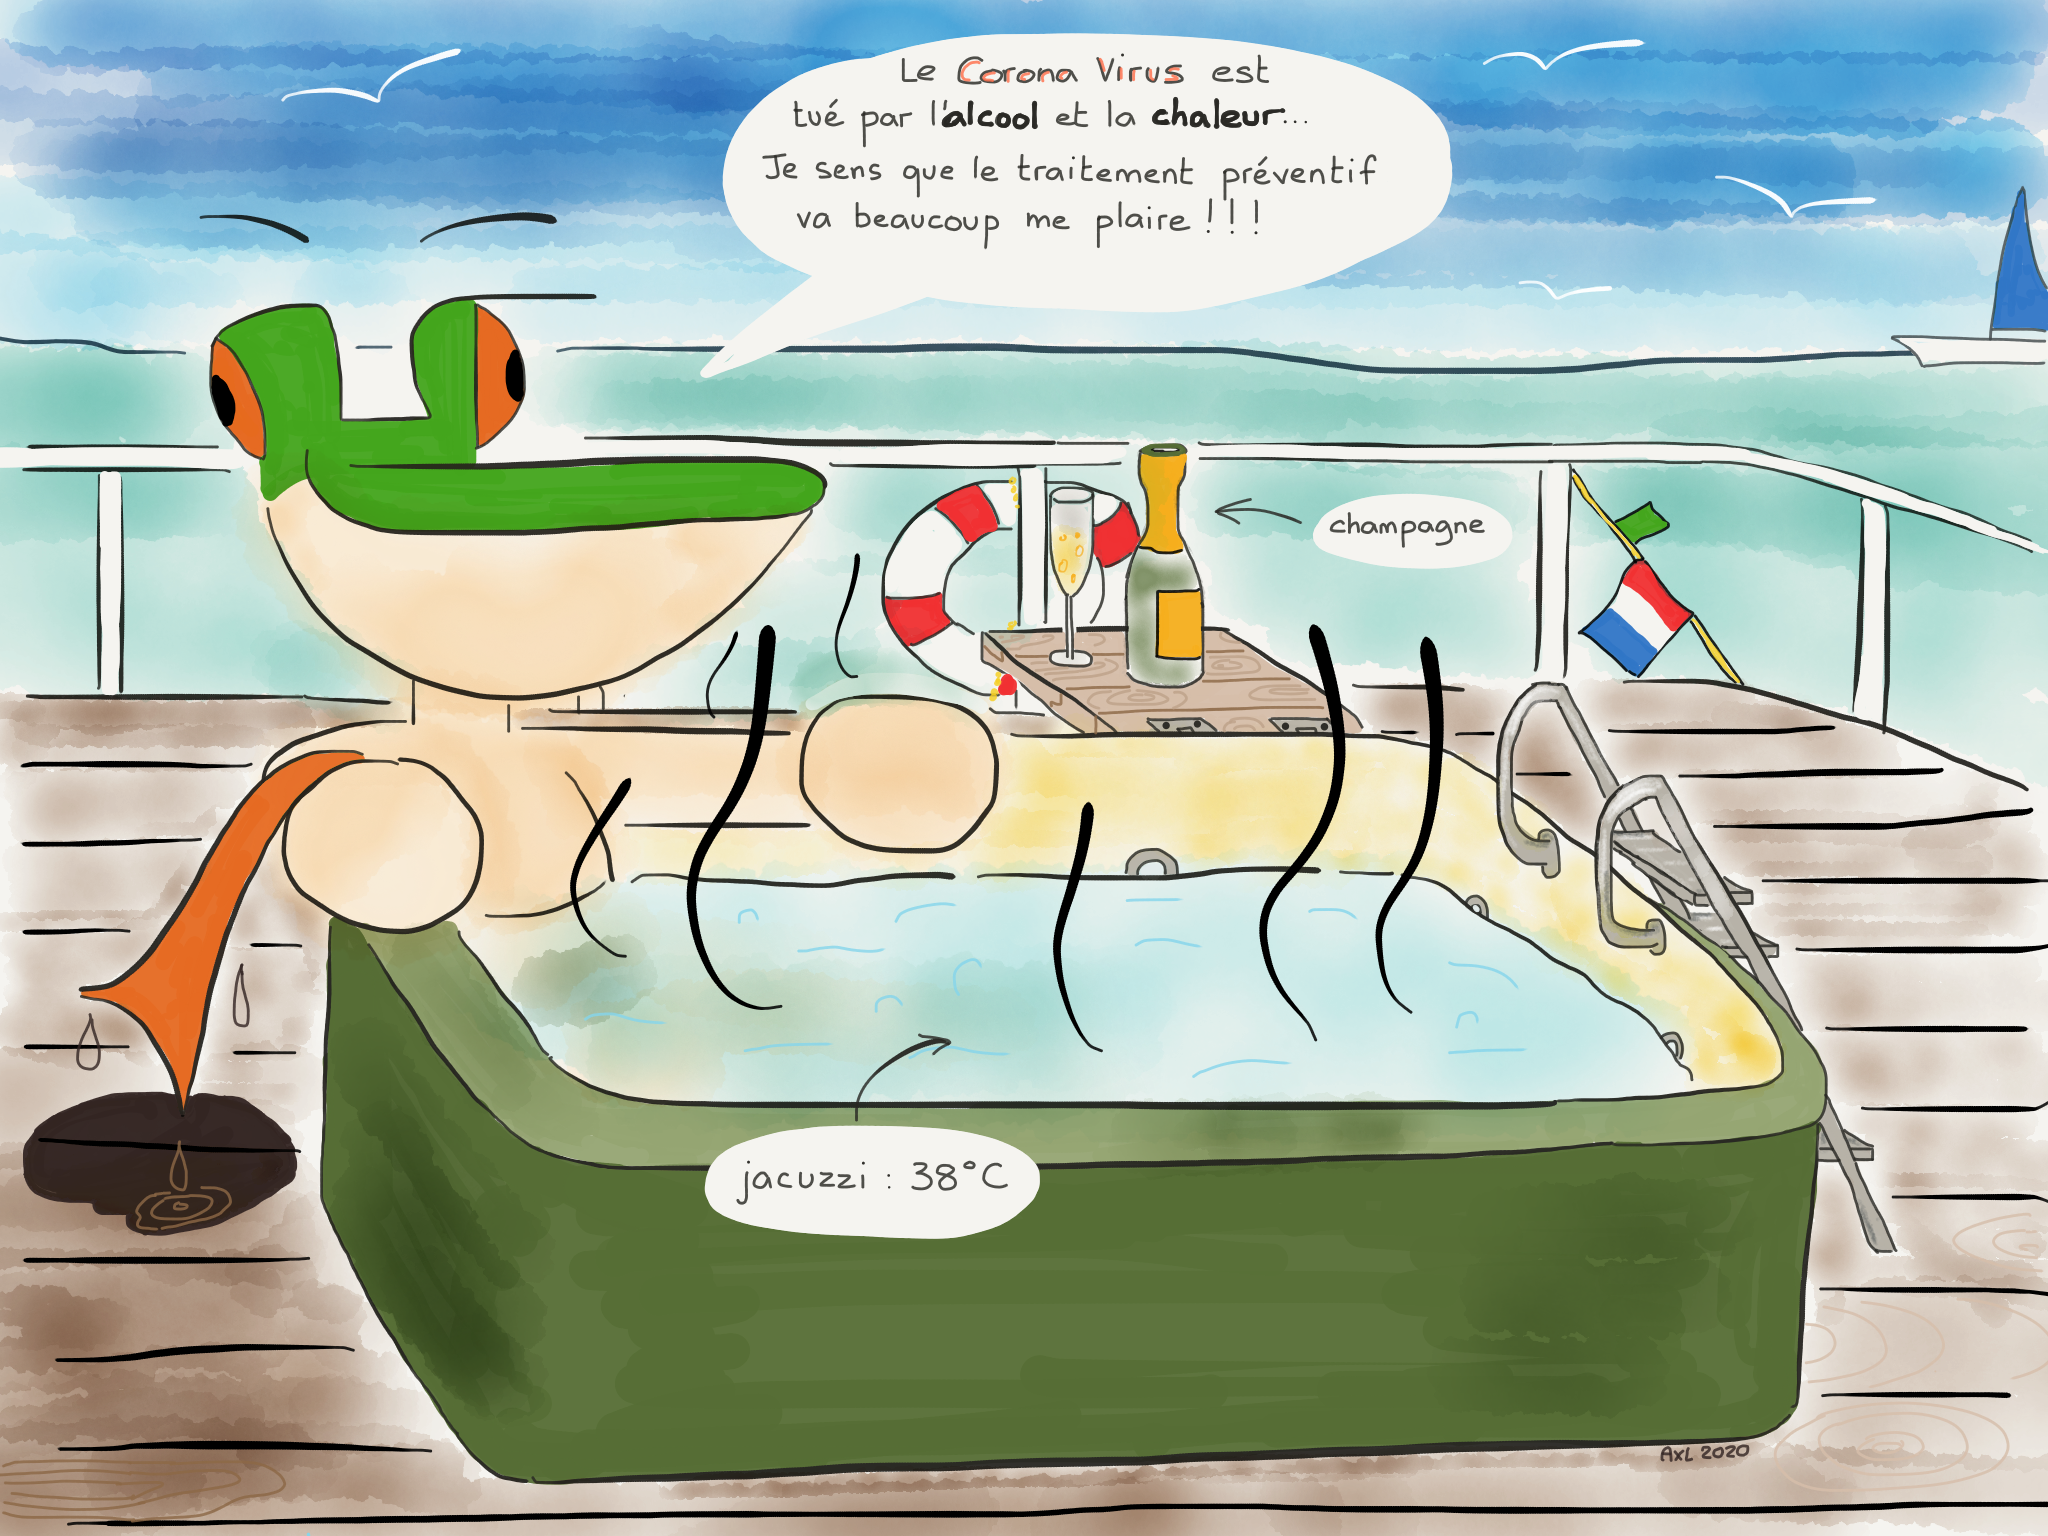
\includegraphics[width=6cm]{./images/2020-03-picocorona.png}\\
  \begin{itemize}

  \item Live Demo: Reverse a Binary with Radare2
  \item Hack into Pico le Croco's apartment
  \item Play Ph0wn challenges
  \end{itemize}

}

\frame{
  \frametitle{Radare2}
  \centering
  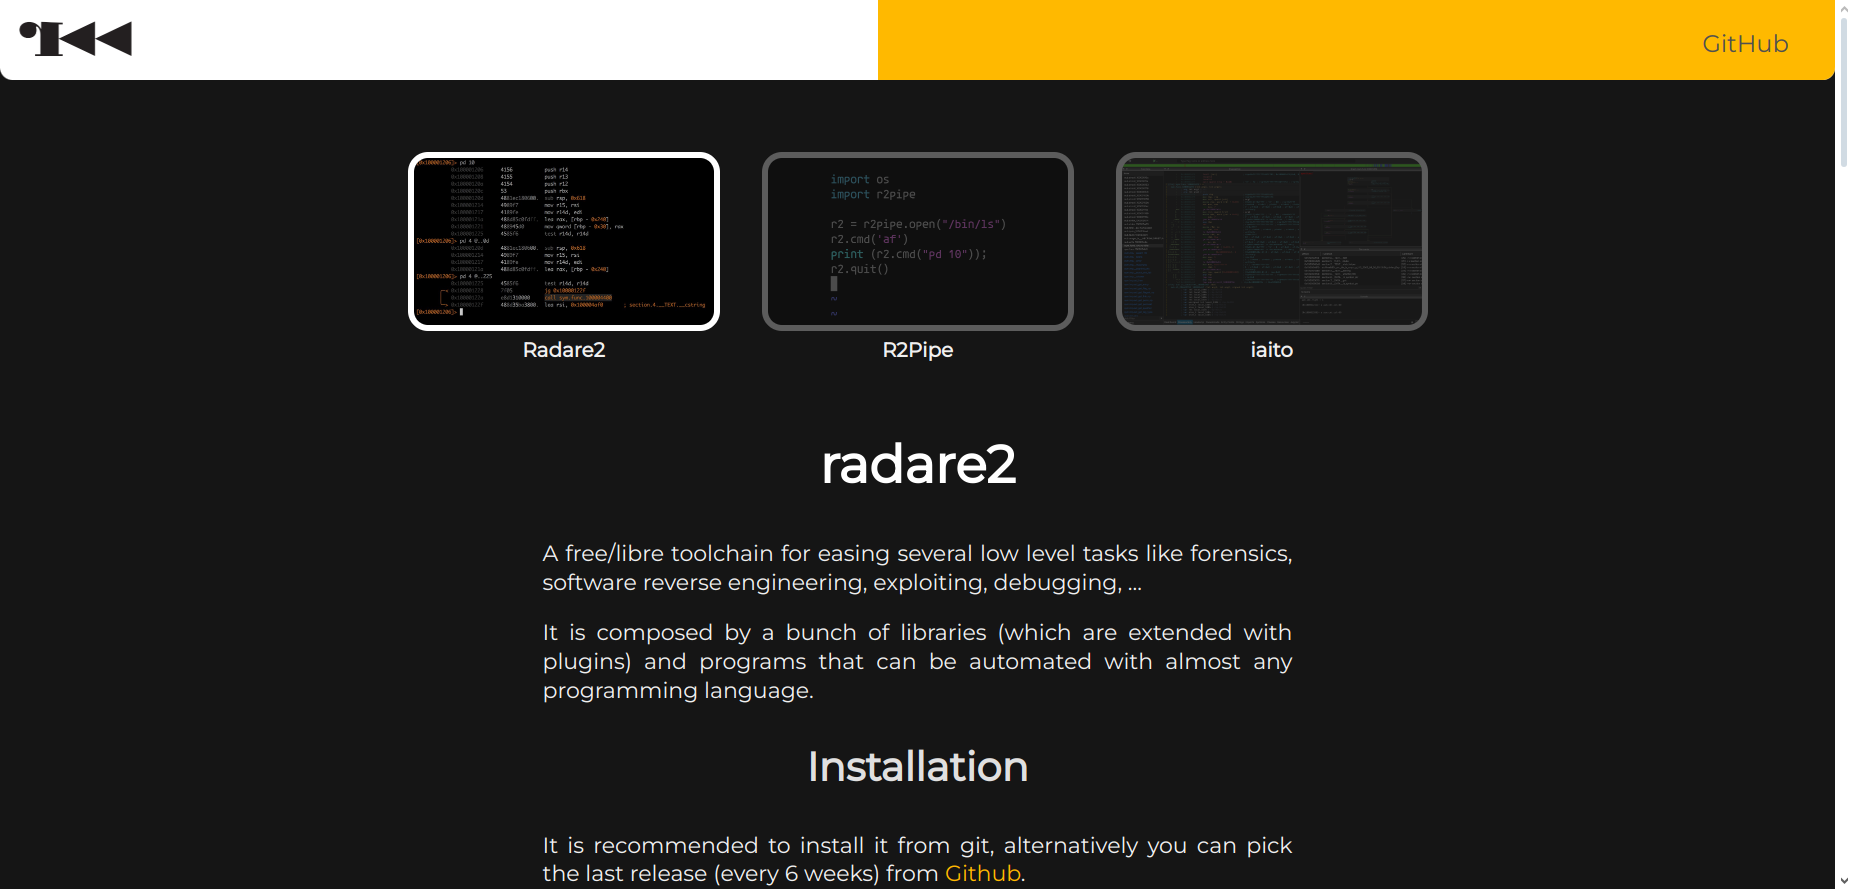
\includegraphics[height=4cm]{./images/radare2.png}\\
  \url{https://www.radare.org/n/radare2.html}

  \begin{itemize}
  \item It's an \textbf{open source disassembler}.
  \item Supports \textbf{many architectures}.
  \item It's \textbf{command-line} based. IDA Pro $=$ \textit{Libre Office}, Radare2 $=$ \textit{vim}.
  \item It's \textit{scriptable}. 
  \end{itemize}
}


\frame{
  \frametitle{Links}
  \centering
  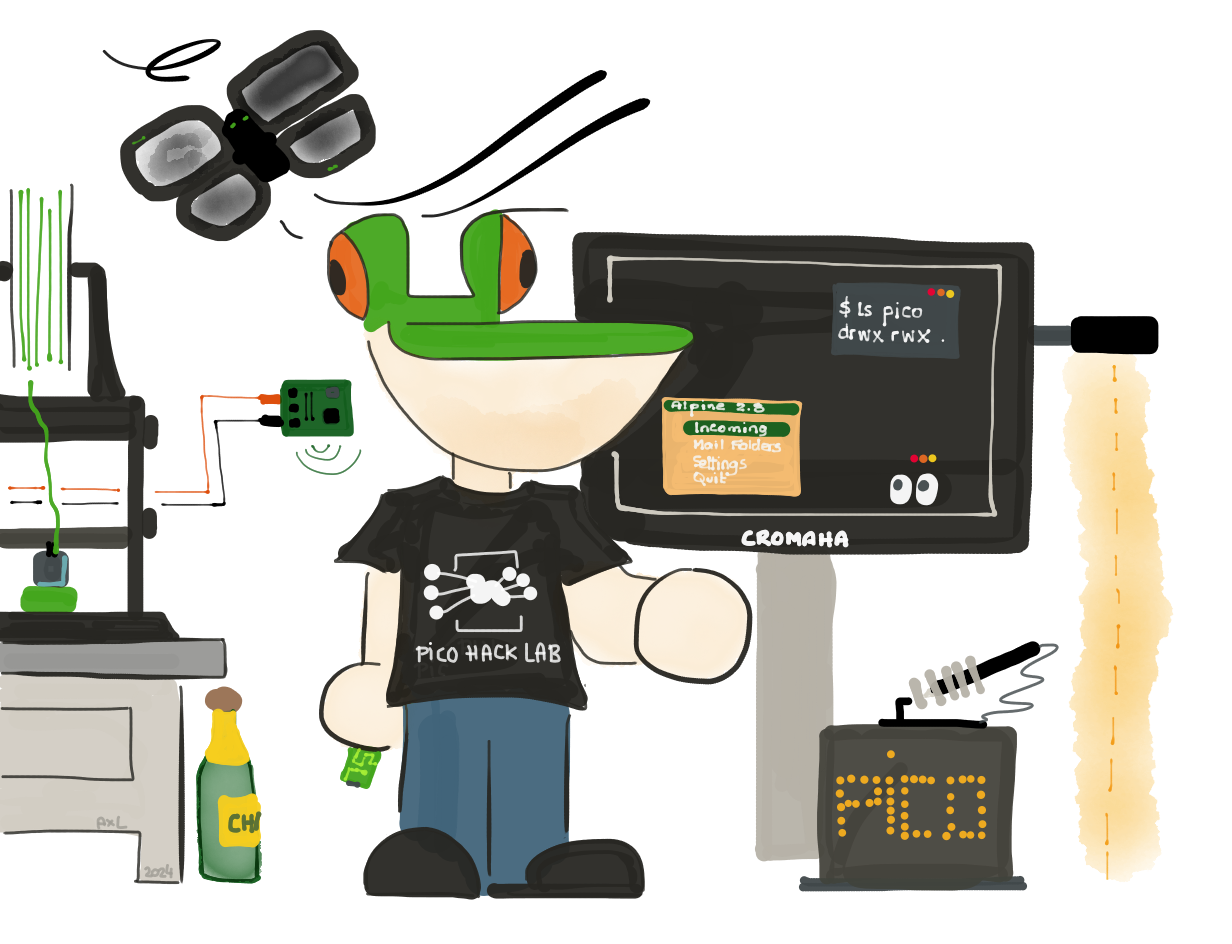
\includegraphics[height=4cm]{../../images/pico-at-shl.png}\\
  \begin{itemize}

  \item \url{https://github.com/SophiaHackLab/ph0wnlabs}
  \item \url{https://ph0wn.shl.contact/}
  \item \url{https://ph0wn.org}
  \item \url{https://cryptax.github.io}
  \item \url{https://pico.masdescrocodiles.fr}

  \end{itemize}
}



\end{document}
